
%% bare_jrnl_compsoc.tex
%% V1.3
%% 2007/01/11
%% by Michael Shell
%% See:
%% http://www.michaelshell.org/
%% for current contact information.
%%
%% This is a skeleton file demonstrating the use of IEEEtran.cls
%% (requires IEEEtran.cls version 1.7 or later) with an IEEE Computer
%% Society journal paper.
%%
%% Support sites:
%% http://www.michaelshell.org/tex/ieeetran/
%% http://www.ctan.org/tex-archive/macros/latex/contrib/IEEEtran/
%% and
%% http://www.ieee.org/

%%*************************************************************************
%% Legal Notice:
%% This code is offered as-is without any warranty either expressed or
%% implied; without even the implied warranty of MERCHANTABILITY or
%% FITNESS FOR A PARTICULAR PURPOSE! 
%% User assumes all risk.
%% In no event shall IEEE or any contributor to this code be liable for
%% any damages or losses, including, but not limited to, incidental,
%% consequential, or any other damages, resulting from the use or misuse
%% of any information contained here.
%%
%% All comments are the opinions of their respective authors and are not
%% necessarily endorsed by the IEEE.
%%
%% This work is distributed under the LaTeX Project Public License (LPPL)
%% ( http://www.latex-project.org/ ) version 1.3, and may be freely used,
%% distributed and modified. A copy of the LPPL, version 1.3, is included
%% in the base LaTeX documentation of all distributions of LaTeX released
%% 2003/12/01 or later.
%% Retain all contribution notices and credits.
%% ** Modified files should be clearly indicated as such, including  **
%% ** renaming them and changing author support contact information. **
%%
%% File list of work: IEEEtran.cls, IEEEtran_HOWTO.pdf, bare_adv.tex,
%%                    bare_conf.tex, bare_jrnl.tex, bare_jrnl_compsoc.tex
%%*************************************************************************

% *** Authors should verify (and, if needed, correct) their LaTeX system  ***
% *** with the testflow diagnostic prior to trusting their LaTeX platform ***
% *** with production work. IEEE's font choices can trigger bugs that do  ***
% *** not appear when using other class files.                            ***
% The testflow support page is at:
% http://www.michaelshell.org/tex/testflow/




% Note that the a4paper option is mainly intended so that authors in
% countries using A4 can easily print to A4 and see how their papers will
% look in print - the typesetting of the document will not typically be
% affected with changes in paper size (but the bottom and side margins will).
% Use the testflow package mentioned above to verify correct handling of
% both paper sizes by the user's LaTeX system.
%
% Also note that the "draftcls" or "draftclsnofoot", not "draft", option
% should be used if it is desired that the figures are to be displayed in
% draft mode.
%
% The Computer Society usually requires 12pt for submissions.
%
\documentclass[12pt,journal,compsoc]{IEEEtran}
%
% If IEEEtran.cls has not been installed into the LaTeX system files,
% manually specify the path to it like:
% \documentclass[12pt,journal,compsoc]{../sty/IEEEtran}



\usepackage{hyperref}

% Some very useful LaTeX packages include:
% (uncomment the ones you want to load)


% *** MISC UTILITY PACKAGES ***
%
%\usepackage{ifpdf}
% Heiko Oberdiek's ifpdf.sty is very useful if you need conditional
% compilation based on whether the output is pdf or dvi.
% usage:
% \ifpdf
%   % pdf code
% \else
%   % dvi code
% \fi
% The latest version of ifpdf.sty can be obtained from:
% http://www.ctan.org/tex-archive/macros/latex/contrib/oberdiek/
% Also, note that IEEEtran.cls V1.7 and later provides a builtin
% \ifCLASSINFOpdf conditional that works the same way.
% When switching from latex to pdflatex and vice-versa, the compiler may
% have to be run twice to clear warning/error messages.






% *** CITATION PACKAGES ***
%
\ifCLASSOPTIONcompsoc
  % IEEE Computer Society needs nocompress option
  % requires cite.sty v4.0 or later (November 2003)
  % \usepackage[nocompress]{cite}
\else
  % normal IEEE
  % \usepackage{cite}
\fi
% cite.sty was written by Donald Arseneau
% V1.6 and later of IEEEtran pre-defines the format of the cite.sty package
% \cite{} output to follow that of IEEE. Loading the cite package will
% result in citation numbers being automatically sorted and properly
% "compressed/ranged". e.g., [1], [9], [2], [7], [5], [6] without using
% cite.sty will become [1], [2], [5]--[7], [9] using cite.sty. cite.sty's
% \cite will automatically add leading space, if needed. Use cite.sty's
% noadjust option (cite.sty V3.8 and later) if you want to turn this off.
% cite.sty is already installed on most LaTeX systems. Be sure and use
% version 4.0 (2003-05-27) and later if using hyperref.sty. cite.sty does
% not currently provide for hyperlinked citations.
% The latest version can be obtained at:
% http://www.ctan.org/tex-archive/macros/latex/contrib/cite/
% The documentation is contained in the cite.sty file itself.
%
% Note that some packages require special options to format as the Computer
% Society requires. In particular, Computer Society  papers do not use
% compressed citation ranges as is done in typical IEEE papers
% (e.g., [1]-[4]). Instead, they list every citation separately in order
% (e.g., [1], [2], [3], [4]). To get the latter we need to load the cite
% package with the nocompress option which is supported by cite.sty v4.0
% and later. Note also the use of a CLASSOPTION conditional provided by
% IEEEtran.cls V1.7 and later.





% *** GRAPHICS RELATED PACKAGES ***
%
\ifCLASSINFOpdf
  % \usepackage[pdftex]{graphicx}
  % declare the path(s) where your graphic files are
  % \graphicspath{{../pdf/}{../jpeg/}}
  % and their extensions so you won't have to specify these with
  % every instance of \includegraphics
  % \DeclareGraphicsExtensions{.pdf,.jpeg,.png}
\else
  % or other class option (dvipsone, dvipdf, if not using dvips). graphicx
  % will default to the driver specified in the system graphics.cfg if no
  % driver is specified.
  % \usepackage[dvips]{graphicx}
  % declare the path(s) where your graphic files are
  % \graphicspath{{../eps/}}
  % and their extensions so you won't have to specify these with
  % every instance of \includegraphics
  % \DeclareGraphicsExtensions{.eps}
\fi
% graphicx was written by David Carlisle and Sebastian Rahtz. It is
% required if you want graphics, photos, etc. graphicx.sty is already
% installed on most LaTeX systems. The latest version and documentation can
% be obtained at: 
% http://www.ctan.org/tex-archive/macros/latex/required/graphics/
% Another good source of documentation is "Using Imported Graphics in
% LaTeX2e" by Keith Reckdahl which can be found as epslatex.ps or
% epslatex.pdf at: http://www.ctan.org/tex-archive/info/
%
% latex, and pdflatex in dvi mode, support graphics in encapsulated
% postscript (.eps) format. pdflatex in pdf mode supports graphics
% in .pdf, .jpeg, .png and .mps (metapost) formats. Users should ensure
% that all non-photo figures use a vector format (.eps, .pdf, .mps) and
% not a bitmapped formats (.jpeg, .png). IEEE frowns on bitmapped formats
% which can result in "jaggedy"/blurry rendering of lines and letters as
% well as large increases in file sizes.
%
% You can find documentation about the pdfTeX application at:
% http://www.tug.org/applications/pdftex





% *** MATH PACKAGES ***
%
%\usepackage[cmex10]{amsmath}
% A popular package from the American Mathematical Society that provides
% many useful and powerful commands for dealing with mathematics. If using
% it, be sure to load this package with the cmex10 option to ensure that
% only type 1 fonts will utilized at all point sizes. Without this option,
% it is possible that some math symbols, particularly those within
% footnotes, will be rendered in bitmap form which will result in a
% document that can not be IEEE Xplore compliant!
%
% Also, note that the amsmath package sets \interdisplaylinepenalty to 10000
% thus preventing page breaks from occurring within multiline equations. Use:
%\interdisplaylinepenalty=2500
% after loading amsmath to restore such page breaks as IEEEtran.cls normally
% does. amsmath.sty is already installed on most LaTeX systems. The latest
% version and documentation can be obtained at:
% http://www.ctan.org/tex-archive/macros/latex/required/amslatex/math/





% *** SPECIALIZED LIST PACKAGES ***
%
\usepackage{algorithmic}
\usepackage[]{algorithm2e}
% algorithmic.sty was written by Peter Williams and Rogerio Brito.
% This package provides an algorithmic environment fo describing algorithms.
% You can use the algorithmic environment in-text or within a figure
% environment to provide for a floating algorithm. Do NOT use the algorithm
% floating environment provided by algorithm.sty (by the same authors) or
% algorithm2e.sty (by Christophe Fiorio) as IEEE does not use dedicated
% algorithm float types and packages that provide these will not provide
% correct IEEE style captions. The latest version and documentation of
% algorithmic.sty can be obtained at:
% http://www.ctan.org/tex-archive/macros/latex/contrib/algorithms/
% There is also a support site at:
% http://algorithms.berlios.de/index.html
% Also of interest may be the (relatively newer and more customizable)
% algorithmicx.sty package by Szasz Janos:
% http://www.ctan.org/tex-archive/macros/latex/contrib/algorithmicx/




% *** ALIGNMENT PACKAGES ***
%
%\usepackage{array}
% Frank Mittelbach's and David Carlisle's array.sty patches and improves
% the standard LaTeX2e array and tabular environments to provide better
% appearance and additional user controls. As the default LaTeX2e table
% generation code is lacking to the point of almost being broken with
% respect to the quality of the end results, all users are strongly
% advised to use an enhanced (at the very least that provided by array.sty)
% set of table tools. array.sty is already installed on most systems. The
% latest version and documentation can be obtained at:
% http://www.ctan.org/tex-archive/macros/latex/required/tools/


%\usepackage{mdwmath}
%\usepackage{mdwtab}
% Also highly recommended is Mark Wooding's extremely powerful MDW tools,
% especially mdwmath.sty and mdwtab.sty which are used to format equations
% and tables, respectively. The MDWtools set is already installed on most
% LaTeX systems. The lastest version and documentation is available at:
% http://www.ctan.org/tex-archive/macros/latex/contrib/mdwtools/


% IEEEtran contains the IEEEeqnarray family of commands that can be used to
% generate multiline equations as well as matrices, tables, etc., of high
% quality.


%\usepackage{eqparbox}
% Also of notable interest is Scott Pakin's eqparbox package for creating
% (automatically sized) equal width boxes - aka "natural width parboxes".
% Available at:
% http://www.ctan.org/tex-archive/macros/latex/contrib/eqparbox/





% *** SUBFIGURE PACKAGES ***
%\ifCLASSOPTIONcompsoc
%\usepackage[tight,normalsize,sf,SF]{subfigure}
%\else
%\usepackage[tight,footnotesize]{subfigure}
%\fi
% subfigure.sty was written by Steven Douglas Cochran. This package makes it
% easy to put subfigures in your figures. e.g., "Figure 1a and 1b". For IEEE
% work, it is a good idea to load it with the tight package option to reduce
% the amount of white space around the subfigures. Computer Society papers
% use a larger font and \sffamily font for their captions, hence the
% additional options needed under compsoc mode. subfigure.sty is already
% installed on most LaTeX systems. The latest version and documentation can
% be obtained at:
% http://www.ctan.org/tex-archive/obsolete/macros/latex/contrib/subfigure/
% subfigure.sty has been superceeded by subfig.sty.


%\ifCLASSOPTIONcompsoc
%  \usepackage[caption=false]{caption}
%  \usepackage[font=normalsize,labelfont=sf,textfont=sf]{subfig}
%\else
%  \usepackage[caption=false]{caption}
%  \usepackage[font=footnotesize]{subfig}
%\fi
% subfig.sty, also written by Steven Douglas Cochran, is the modern
% replacement for subfigure.sty. However, subfig.sty requires and
% automatically loads Axel Sommerfeldt's caption.sty which will override
% IEEEtran.cls handling of captions and this will result in nonIEEE style
% figure/table captions. To prevent this problem, be sure and preload
% caption.sty with its "caption=false" package option. This is will preserve
% IEEEtran.cls handing of captions. Version 1.3 (2005/06/28) and later 
% (recommended due to many improvements over 1.2) of subfig.sty supports
% the caption=false option directly:
\ifCLASSOPTIONcompsoc
  \usepackage[caption=false,font=normalsize,labelfont=sf,textfont=sf]{subfig}
\else
  \usepackage[caption=false,font=footnotesize]{subfig}
\fi
%
% The latest version and documentation can be obtained at:
% http://www.ctan.org/tex-archive/macros/latex/contrib/subfig/
% The latest version and documentation of caption.sty can be obtained at:
% http://www.ctan.org/tex-archive/macros/latex/contrib/caption/




% *** FLOAT PACKAGES ***
%
%\usepackage{fixltx2e}
% fixltx2e, the successor to the earlier fix2col.sty, was written by
% Frank Mittelbach and David Carlisle. This package corrects a few problems
% in the LaTeX2e kernel, the most notable of which is that in current
% LaTeX2e releases, the ordering of single and double column floats is not
% guaranteed to be preserved. Thus, an unpatched LaTeX2e can allow a
% single column figure to be placed prior to an earlier double column
% figure. The latest version and documentation can be found at:
% http://www.ctan.org/tex-archive/macros/latex/base/



%\usepackage{stfloats}
% stfloats.sty was written by Sigitas Tolusis. This package gives LaTeX2e
% the ability to do double column floats at the bottom of the page as well
% as the top. (e.g., "\begin{figure*}[!b]" is not normally possible in
% LaTeX2e). It also provides a command:
%\fnbelowfloat
% to enable the placement of footnotes below bottom floats (the standard
% LaTeX2e kernel puts them above bottom floats). This is an invasive package
% which rewrites many portions of the LaTeX2e float routines. It may not work
% with other packages that modify the LaTeX2e float routines. The latest
% version and documentation can be obtained at:
% http://www.ctan.org/tex-archive/macros/latex/contrib/sttools/
% Documentation is contained in the stfloats.sty comments as well as in the
% presfull.pdf file. Do not use the stfloats baselinefloat ability as IEEE
% does not allow \baselineskip to stretch. Authors submitting work to the
% IEEE should note that IEEE rarely uses double column equations and
% that authors should try to avoid such use. Do not be tempted to use the
% cuted.sty or midfloat.sty packages (also by Sigitas Tolusis) as IEEE does
% not format its papers in such ways.




%\ifCLASSOPTIONcaptionsoff
%  \usepackage[nomarkers]{endfloat}
% \let\MYoriglatexcaption\caption
% \renewcommand{\caption}[2][\relax]{\MYoriglatexcaption[#2]{#2}}
%\fi
% endfloat.sty was written by James Darrell McCauley and Jeff Goldberg.
% This package may be useful when used in conjunction with IEEEtran.cls'
% captionsoff option. Some IEEE journals/societies require that submissions
% have lists of figures/tables at the end of the paper and that
% figures/tables without any captions are placed on a page by themselves at
% the end of the document. If needed, the draftcls IEEEtran class option or
% \CLASSINPUTbaselinestretch interface can be used to increase the line
% spacing as well. Be sure and use the nomarkers option of endfloat to
% prevent endfloat from "marking" where the figures would have been placed
% in the text. The two hack lines of code above are a slight modification of
% that suggested by in the endfloat docs (section 8.3.1) to ensure that
% the full captions always appear in the list of figures/tables - even if
% the user used the short optional argument of \caption[]{}.
% IEEE papers do not typically make use of \caption[]'s optional argument,
% so this should not be an issue. A similar trick can be used to disable
% captions of packages such as subfig.sty that lack options to turn off
% the subcaptions:
% For subfig.sty:
% \let\MYorigsubfloat\subfloat
% \renewcommand{\subfloat}[2][\relax]{\MYorigsubfloat[]{#2}}
% For subfigure.sty:
% \let\MYorigsubfigure\subfigure
% \renewcommand{\subfigure}[2][\relax]{\MYorigsubfigure[]{#2}}
% However, the above trick will not work if both optional arguments of
% the \subfloat/subfig command are used. Furthermore, there needs to be a
% description of each subfigure *somewhere* and endfloat does not add
% subfigure captions to its list of figures. Thus, the best approach is to
% avoid the use of subfigure captions (many IEEE journals avoid them anyway)
% and instead reference/explain all the subfigures within the main caption.
% The latest version of endfloat.sty and its documentation can obtained at:
% http://www.ctan.org/tex-archive/macros/latex/contrib/endfloat/
%
% The IEEEtran \ifCLASSOPTIONcaptionsoff conditional can also be used
% later in the document, say, to conditionally put the References on a 
% page by themselves.




% *** PDF, URL AND HYPERLINK PACKAGES ***
%
%\usepackage{url}
% url.sty was written by Donald Arseneau. It provides better support for
% handling and breaking URLs. url.sty is already installed on most LaTeX
% systems. The latest version can be obtained at:
% http://www.ctan.org/tex-archive/macros/latex/contrib/misc/
% Read the url.sty source comments for usage information. Basically,
% \url{my_url_here}.





% *** Do not adjust lengths that control margins, column widths, etc. ***
% *** Do not use packages that alter fonts (such as pslatex).         ***
% There should be no need to do such things with IEEEtran.cls V1.6 and later.
% (Unless specifically asked to do so by the journal or conference you plan
% to submit to, of course. )

\usepackage{graphicx}

% correct bad hyphenation here
\hyphenation{op-tical net-works semi-conduc-tor}


\begin{document}
%
% paper title
% can use linebreaks \\ within to get better formatting as desired
\title{Schizophrenia classification using \\multi-scale functional connectivity }
%
%
% author names and IEEE memberships
% note positions of commas and nonbreaking spaces ( ~ ) LaTeX will not break
% a structure at a ~ so this keeps an author's name from being broken across
% two lines.
% use \thanks{} to gain access to the first footnote area
% a separate \thanks must be used for each paragraph as LaTeX2e's \thanks
% was not built to handle multiple paragraphs
%
%
%\IEEEcompsocitemizethanks is a special \thanks that produces the bulleted
% lists the Computer Society journals use for "first footnote" author
% affiliations. Use \IEEEcompsocthanksitem which works much like \item
% for each affiliation group. When not in compsoc mode,
% \IEEEcompsocitemizethanks becomes like \thanks and
% \IEEEcompsocthanksitem becomes a line break with idention. This
% facilitates dual compilation, although admittedly the differences in the
% desired content of \author between the different types of papers makes a
% one-size-fits-all approach a daunting prospect. For instance, compsoc 
% journal papers have the author affiliations above the "Manuscript
% received ..."  text while in non-compsoc journals this is reversed. Sigh.

\author{Christian~Dansereau% <-this % stops a space
\IEEEcompsocitemizethanks{\IEEEcompsocthanksitem Mr. Dansereau is with the Department
of Computer science, University of Montreal, Montreal,
CA.\protect\\
% note need leading \protect in front of \\ to get a newline within \thanks as
% \\ is fragile and will error, could use \hfil\break instead.
E-mail: christiandansereau@gmail.com}% <-this % stops a space
\thanks{Manuscript received April 28, 2015}}

% note the % following the last \IEEEmembership and also \thanks - 
% these prevent an unwanted space from occurring between the last author name
% and the end of the author line. i.e., if you had this:
% 
% \author{....lastname \thanks{...} \thanks{...} }
%                     ^------------^------------^----Do not want these spaces!
%
% a space would be appended to the last name and could cause every name on that
% line to be shifted left slightly. This is one of those "LaTeX things". For
% instance, "\textbf{A} \textbf{B}" will typeset as "A B" not "AB". To get
% "AB" then you have to do: "\textbf{A}\textbf{B}"
% \thanks is no different in this regard, so shield the last } of each \thanks
% that ends a line with a % and do not let a space in before the next \thanks.
% Spaces after \IEEEmembership other than the last one are OK (and needed) as
% you are supposed to have spaces between the names. For what it is worth,
% this is a minor point as most people would not even notice if the said evil
% space somehow managed to creep in.



% The paper headers
\markboth{Project 2 IFT6141 Winter~2015}%
{Shell \MakeLowercase{\textit{et al.}}: Bare Demo of IEEEtran.cls for Computer Society Journals}
% The only time the second header will appear is for the odd numbered pages
% after the title page when using the twoside option.
% 
% *** Note that you probably will NOT want to include the author's ***
% *** name in the headers of peer review papers.                   ***
% You can use \ifCLASSOPTIONpeerreview for conditional compilation here if
% you desire.



% The publisher's ID mark at the bottom of the page is less important with
% Computer Society journal papers as those publications place the marks
% outside of the main text columns and, therefore, unlike regular IEEE
% journals, the available text space is not reduced by their presence.
% If you want to put a publisher's ID mark on the page you can do it like
% this:
%\IEEEpubid{0000--0000/00\$00.00~\copyright~2007 IEEE}
% or like this to get the Computer Society new two part style.
%\IEEEpubid{\makebox[\columnwidth]{\hfill 0000--0000/00/\$00.00~\copyright~2007 IEEE}%
%\hspace{\columnsep}\makebox[\columnwidth]{Published by the IEEE Computer Society\hfill}}
% Remember, if you use this you must call \IEEEpubidadjcol in the second
% column for its text to clear the IEEEpubid mark (Computer Society jorunal
% papers don't need this extra clearance.)



% use for special paper notices
%\IEEEspecialpapernotice{(Invited Paper)}



% for Computer Society papers, we must declare the abstract and index terms
% PRIOR to the title within the \IEEEcompsoctitleabstractindextext IEEEtran
% command as these need to go into the title area created by \maketitle.
\IEEEcompsoctitleabstractindextext{%
\begin{abstract}
%\boldmath
The objective of Project 2 is to explore if feature selection based on a margin maximisation criteria would improve the performance of a classification model applied on neuro-imaging data. During the project we have explored normalization procedure and the proper pipeline to identify the right model and parameters.

\end{abstract}
% IEEEtran.cls defaults to using nonbold math in the Abstract.
% This preserves the distinction between vectors and scalars. However,
% if the journal you are submitting to favors bold math in the abstract,
% then you can use LaTeX's standard command \boldmath at the very start
% of the abstract to achieve this. Many IEEE journals frown on math
% in the abstract anyway. In particular, the Computer Society does
% not want either math or citations to appear in the abstract.

% Note that keywords are not normally used for peerreview papers.
\begin{IEEEkeywords}
Schizophrenia, classification, multiscale, feature selection.
\end{IEEEkeywords}}


% make the title area
\maketitle


% To allow for easy dual compilation without having to reenter the
% abstract/keywords data, the \IEEEcompsoctitleabstractindextext text will
% not be used in maketitle, but will appear (i.e., to be "transported")
% here as \IEEEdisplaynotcompsoctitleabstractindextext when compsoc mode
% is not selected <OR> if conference mode is selected - because compsoc
% conference papers position the abstract like regular (non-compsoc)
% papers do!
\IEEEdisplaynotcompsoctitleabstractindextext
% \IEEEdisplaynotcompsoctitleabstractindextext has no effect when using
% compsoc under a non-conference mode.


% For peer review papers, you can put extra information on the cover
% page as needed:
% \ifCLASSOPTIONpeerreview
% \begin{center} \bfseries EDICS Category: 3-BBND \end{center}
% \fi
%
% For peerreview papers, this IEEEtran command inserts a page break and
% creates the second title. It will be ignored for other modes.
\IEEEpeerreviewmaketitle



\section{Introduction}
% Computer Society journal papers do something a tad strange with the very
% first section heading (almost always called "Introduction"). They place it
% ABOVE the main text! IEEEtran.cls currently does not do this for you.
% However, You can achieve this effect by making LaTeX jump through some
% hoops via something like:
%
%\ifCLASSOPTIONcompsoc
%  \noindent\raisebox{2\baselineskip}[0pt][0pt]%
%  {\parbox{\columnwidth}{\section{Introduction}\label{sec:introduction}%
%  \global\everypar=\everypar}}%
%  \vspace{-1\baselineskip}\vspace{-\parskip}\par
%\else
%  \section{Introduction}\label{sec:introduction}\par
%\fi
%
% Admittedly, this is a hack and may well be fragile, but seems to do the
% trick for me. Note the need to keep any \label that may be used right
% after \section in the above as the hack puts \section within a raised box.


% The very first letter is a 2 line initial drop letter followed
% by the rest of the first word in caps (small caps for compsoc).
% 
% form to use if the first word consists of a single letter:
% \IEEEPARstart{A}{demo} file is ....
% 
% form to use if you need the single drop letter followed by
% normal text (unknown if ever used by IEEE):
% \IEEEPARstart{A}{}demo file is ....
% 
% Some journals put the first two words in caps:
% \IEEEPARstart{T}{his demo} file is ....
% 
% Here we have the typical use of a "T" for an initial drop letter
% and "HIS" in caps to complete the first word.



\IEEEPARstart{T}{he} use of machine learning algorithm in the context of neuroimaging is new and pose multiple constrains, like in any other biomedical dataset we are faced with a large number of features and a small number of examples (the number of subjects). Support vector machine (SVM) \cite{Cortes1995} are attempting to find an hyperplane that will maximize the margin between two classes. To do so SVM use support vectors that are basically representative example. In this paper we are attempting to discriminate two population control subject and patient with Schizophrenia. In order to do so we are recording the brain activity of each individual using a functional magnetic resonance imaging (fMRI) machine. This modality give use a 3D snapshot of the brain activity every 2.5 second. A popular metric to evaluate brain activity pathern is to use connectivity metrics like the temporal correlation of every pair of grey matter region in the brain.

% You must have at least 2 lines in the paragraph with the drop letter
% (should never be an issue)

%\hfill mds
%\hfill January 11, 2015

\subsection{Objectives}
The objectives of the projects are the following: 1) Normalize the data and account for confounding variables; 2) find if there is a functional scale more optimal for classification of the problem at hand; 3) Evaluate the performance of the retained pipeline for in a multi-scale analysis and assess if a boost in performance can be achieved by combining multiple functional scales using a variation of the bagging algorithm; 4) and finality implement and use a margin optimization algorithm for feature selection applied to functional neuro-imaging data.

\subsection{Public code and data}
The code used in this experiment is available on a 
GitHub repository at the following URL: \url{https://github.com/cdansereau/vision_or/code_project2}. A IPython Notebook is also provided with all of the figure generation scripts.


% needed in second column of first page if using \IEEEpubid
%\IEEEpubidadjcol

%\subsubsection{Subsubsection Heading Here}
%Subsubsection text here.


% An example of a floating figure using the graphicx package.
% Note that \label must occur AFTER (or within) \caption.
% For figures, \caption should occur after the \includegraphics.
% Note that IEEEtran v1.7 and later has special internal code that
% is designed to preserve the operation of \label within \caption
% even when the captionsoff option is in effect. However, because
% of issues like this, it may be the safest practice to put all your
% \label just after \caption rather than within \caption{}.
%
% Reminder: the "draftcls" or "draftclsnofoot", not "draft", class
% option should be used if it is desired that the figures are to be
% displayed while in draft mode.
%





% An example of a double column floating figure using two subfigures.
% (The subfig.sty package must be loaded for this to work.)
% The subfigure \label commands are set within each subfloat command, the
% \label for the overall figure must come after \caption.
% \hfil must be used as a separator to get equal spacing.
% The subfigure.sty package works much the same way, except \subfigure is
% used instead of \subfloat.
%
%\begin{figure}[!t]
%\centerline{
%\subfloat[Case I]
%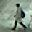
\includegraphics[width=2.5in]{015_1.jpg}%
%\label{fig_first_case}
%}
%\vfil
%\subfloat[Case II]{
%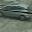
\includegraphics[width=2.5in]{038_3.jpg}%
%\label{fig_second_case}
%}
%
%\caption{Simulation results}
%\label{fig_sim}
%}
%\end{figure}
%
% Note that often IEEE papers with subfigures do not employ subfigure
% captions (using the optional argument to \subfloat), but instead will
% reference/describe all of them (a), (b), etc., within the main caption.


% An example of a floating table. Note that, for IEEE style tables, the 
% \caption command should come BEFORE the table. Table text will default to
% \footnotesize as IEEE normally uses this smaller font for tables.
% The \label must come after \caption as always.
%
%\begin{table}[!t]
%% increase table row spacing, adjust to taste
%\renewcommand{\arraystretch}{1.3}
% if using array.sty, it might be a good idea to tweak the value of
% \extrarowheight as needed to properly center the text within the cells
%\caption{An Example of a Table}
%\label{table_example}
%\centering
%% Some packages, such as MDW tools, offer better commands for making tables
%% than the plain LaTeX2e tabular which is used here.
%\begin{tabular}{|c||c|}
%\hline
%One & Two\\
%\hline
%Three & Four\\
%\hline
%\end{tabular}
%\end{table}


% Note that IEEE does not put floats in the very first column - or typically
% anywhere on the first page for that matter. Also, in-text middle ("here")
% positioning is not used. Most IEEE journals use top floats exclusively.
% However, Computer Society journals sometimes do use bottom floats - bear
% this in mind when choosing appropriate optional arguments for the
% figure/table environments.
% Note that, LaTeX2e, unlike IEEE journals, places footnotes above bottom
% floats. This can be corrected via the \fnbelowfloat command of the
% stfloats package.


\section{Method}
The project was realized in python with the following libraries: scipy \cite{scipy}, scikit-learn \cite{scikitlearn} and matplotlib \cite{matplotlib}.

\subsection{Dataset}
The dataset used in this paper is the COBRE (The Center for Biomedical Research Excellence) dataset from the indi initiative. It consist of raw anatomical and functional MR data from 72 patients with Schizophrenia and 75 healthy controls (ages ranging from 18 to 65 in each group). All subjects were screened and excluded if they had; history of neurological disorder, history of mental retardation, history of severe head trauma with more than 5 minutes loss of consciousness, history of substance abuse or dependence within the last 12 months. Diagnostic information was collected using the Structured Clinical Interview used for DSM Disorders (SCID).

A multi-echo MPRAGE (MEMPR) sequence was used with the following parameters: TR/TE/TI = 2530/[1.64, 3.5, 5.36, 7.22, 9.08]/900 ms, flip angle = 7°, FOV = 256x256 mm, Slab thickness = 176 mm, Matrix = 256x256x176, Voxel size =1x1x1 mm, Number of echos = 5, Pixel bandwidth =650 Hz, Total scan time = 6 min. With 5 echoes, the TR, TI and time to encode partitions for the MEMPR are similar to that of a conventional MPRAGE, resulting in similar GM/WM/CSF contrast.

Rest data was collected with single-shot full k-space echo-planar imaging (EPI) with ramp sampling correction using the intercomissural line (AC-PC) as a reference (TR: 2 s, TE: 29 ms, matrix size: 64x64, 32 slices, voxel size: 3x3x4 mm3).

Phenotypic data available for every participant: gender, age, handedness and diagnostic information (control subject of patient with Schizophrenia).
An official description of the data and a publicly available version of the dataset is available on the NITRC \footnote{\url{http://fcon_1000.projects.nitrc.org/indi/retro/cobre.html}} website.


\subsection{Preprocessing and feature extraction}
The datasets were analysed using the NeuroImaging Analysis Kit (NIAK\footnote{\url{http://www.nitrc.org/projects/niak/}}) version 0.12.14, under CentOS version 6.3 with Octave\footnote{\url{http://gnu.octave.org}} version 3.8.1 and the Minc toolkit\footnote{\url{http://www.bic.mni.mcgill.ca/ServicesSoftware/ServicesSoftwareMincToolKit}} version 0.3.18. Analyses were executed in parallel on the "Mammouth" supercomputer\footnote{\url{http://www.calculquebec.ca/index.php/en/resources/compute-servers/mammouth-parallele-ii}}, using the pipeline system for Octave and Matlab \cite{Bellec2010}, version 1.0.2. Brain map visualizations were created using MRICron software \cite{Rorden2007}. Each fMRI dataset was corrected of inter-slice difference in acquisition time and the parameters of a rigid-body motion was estimated for each time frame. Rigid-body motion was estimated within as well as between runs, using the median volume of the first run as a target. The median volume of one selected fMRI run for each subject was coregistered with a T1 individual scan using Minctracc \cite{Collins1998}, which was itself non-linearly transformed to the Montreal Neurological Institute (MNI) template \cite{Fonov2011} using the CIVET pipeline \cite{Zijdenbos2002}. The MNI symmetric template was generated from the ICBM152 sample of 152 young adults, after 40 iterations of non-linear coregistration. The rigid-body transform, fMRI-to-T1 transform and T1-to-stereotaxic transform were all combined, and the functional volumes were resampled in the MNI space at a 3 mm isotropic resolution. The a censoring method described in \cite{Power2012} called "scrubbing" was used to remove the volumes with excessive motion using a cut-off value of $FD\geq0.5$. A minimum number of 50 unscrubbed volumes per run, corresponding to $\sim 125$ s of acquisition for a TR of 2.5 seconds, was then required for further analysis. The following nuisance parameters were regressed out from the time series at each voxel: slow time drifts (basis of discrete cosines with a 0.01 Hz high-pass cut-off), average signals in conservative masks of the white matter and the lateral ventricles as well as the first principal components (95\% energy) of the six rigid-body motion parameters and their squares \cite{Lund2006},\cite{Giove2009}. The fMRI volumes were finally spatially smoothed with a 6 mm isotropic Gaussian blurring kernel. 

Functional connectivity matrices were obtained from 9 scales using a functional template based on an independent dataset of $\sim 200$ subjects form the 1000 functional connectome project (Cambridge dataset). The 9 scales were obtain using the BASC pipeline \cite{Bellec2010a} which is a unsupervised bootstrap clustering procedure for automatic detection of functional scales based on a stability criteria. resulting in 9 partitions of the brain in 7, 12, 20, 36, 64, 122, 197, 325, 444 networks see Figure \ref{fig_connectomes3x3} for an example of the the resulting connectome of one subject.

\begin{figure}[h]
\centering
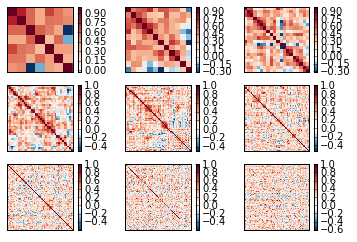
\includegraphics[width=8cm]{connectome3x3.png}
\caption{Exemple of the connectomes for one subject at scale 7, 12, 20, 36, 64, 122, 197, 325 and 444.}
\label{fig_connectomes3x3}
\end{figure}

\subsection{Calibrating the problem}

Has a first step we need to assess the difficulty of the classification task at hand and to do so we are throwing our problem to a simple off the shelf model with the default parameter. This will define the complexity of the problem. In our case we have used scales 64 which will give us a good reference point in term of the problem complexity. The initial classifier model used was a linear SVM with parameter fixed to $C=1$ (the default value). In all the subsequent analysis we are performing a stratified 10-fold cross-validation and include a parameter in the SVM classifier to account for the unbalance dataset by automatically re-weight each class by the inverse of its frequency.

The next step is to find the most adapted hyper-parameters (C and/or Gamma if using Gaussian kernel) for our classification problem we choose to use a grid search approach. The grid search parametrised as follow for C ($10^-2$ to $10^3$) and for Gamma ($10^-5$ to $10^1$) The grid search and the final classification were evaluated using a stratified cross-validation due to the unbalanced number of examples available for each class.


\subsection{Preprocessing and confounds regression}

SVM is sensitive to not normalized data we therefore normalize the features of each subject to zero mean and unit variance. Since some bias can be introduce by confounding factors we account for them by regressing the age and gender contribution based on the training set.


\subsection{Optimal functional scale}
The fact that we are looking at various level of data abstraction due to the clustering process of BASC in functional scales, we may be more sensitive at some particular scale than other for a given pathology. We have therefore tested the model for each of the 9 scales.

\subsection{Multiscale bagging predictions}
The idea in this case was to combine the vote of the classifier at each scale using a bagging approach. This ensemble approach combine the predictor of each scale in a bagging procedure as illustrated in Figure \ref{fig_bagging_multiscale}. We simple take a majority vote from all the classifier. Contrary to most ensemble methods this case may be sensitive to scale that do not have sufficient information to yield a good prediction we therefore took a subset of the scales based on the individual performance obtain in Figure \ref{fig_scale_svm}.

\begin{figure}[h]
\centering
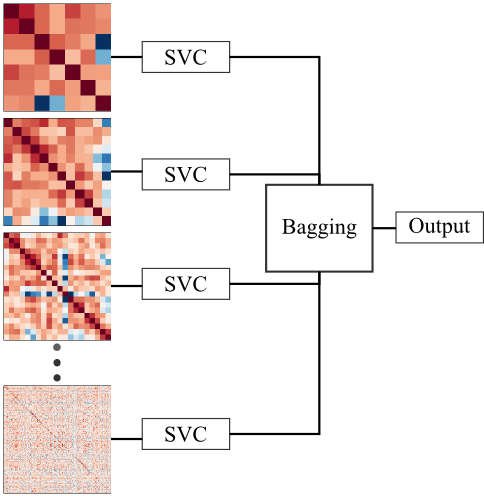
\includegraphics[width=8cm]{bagging_multiscale.png}
\caption{Pipeline of the modified bagging procedure using multi-scale functional connectomes.}
\label{fig_bagging_multiscale}
\end{figure}

\subsection{I-Relief margin optimization}
\cite{Gilad-bachrach2004} describe feature selection as "the task of choosing a small set out of a given set of features that capture the relevant properties of the data". In our supervised classification problems the relevance is determined by the labels on the training data. The choice of the features is therefore essential to obtain a compact and accurate classifier. When using an SVM classifier an intuitive question may arise regarding the objective of a support vector machine,  it attempt to find the hyperplane that maximize the margin between two classes in a binary task and we can hypothesis that it may exist a subset of feature that optimally discriminate the two classes. If such a subset exist it would 1) be very informative in term of the clinical interpretation and 2) it would potentially require less support vectors and therefore less examples. In order to measure the quality of sets of features a greedy algorithm proposed by \cite{Gilad-bachrach2004} and illustrated in Algorithm \ref{algo_gflip} do iteratively a search of the optimal set of feature by adding and/or removing a feature to/from the subset.

\begin{algorithm}
\caption{Greedy feature flip}
\begin{algorithmic} 
\STATE Init set of chosen features $F = \emptyset$
\FOR{$t=1,2,...$}
\STATE pick a random permutation s of ${1...N}$
\FOR{$i=$ 1 to N}
\STATE $e_{1}=e(F\cup{s(i)})$
\STATE $e_{2}=e(F\setminus{s(i)})$
\IF{$e_{1}>e_{2}$}
\STATE $F=F\cup{s(i)}$
\ELSE
\STATE $F=F\setminus{s(i)}$
\ENDIF
\ENDFOR
\STATE if no change made in last step then break
\ENDFOR
\end{algorithmic}
\label{algo_gflip}
\end{algorithm}

Unfortunately the greedy version is not practical for problems with a large feature space like ours we therefore need an alternative. To our knowledge two papers have proposed an online iterative algorithm \cite{Gilad-bachrach2004} and \cite{Sun2007} that aim at maximizing the margin. We have used an implementation of I-Relief from the package \cite{Hanke2009} originally proposed by \cite{Sun2007} in order to evaluate the potential of this technique.

This procedure give use a weight for each feature we then select the feature with the largest weights. since we do not know the number of features to select we propose to search for the best set based on a nested cross-validation with the criteria to select the best based on how much there weight diverge from the average weight. We search on an standard deviation range of $\alpha\in{0...2.75}$ with a step of 0.25. The threshold that we will use to to include all the features that obtained a weight greater or equal to $W_{threshold}$ is defined as $W_{threshold} = W_{std}*\alpha+\overline{\rm W}$.


\section{Results}

\subsection{Calibrating the problem}

 The figure \ref{fig_calib_svm} show the performance of the off the shelf model and we obtained 64.53\% with an AUC of 0.70.
 
\begin{figure}[h]
\centering
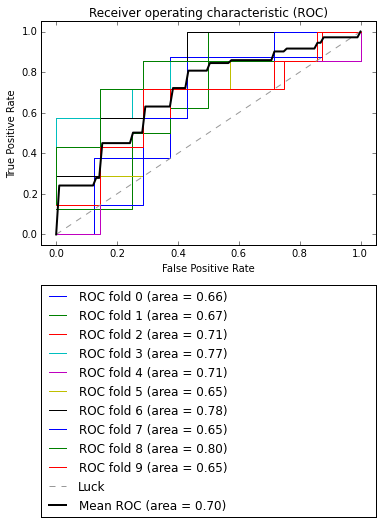
\includegraphics[width=8cm]{svc_linear_calibration_scale64x64.png}
\caption{Calibration of the classification task: Receiver operating characteristic (ROC) curve of the 10 fold cross validation with the average of ROC curve. The legend show the respective AUC (area under the curve) of each fold and the average AUC. The accuracy obtained was 64.53\%.}
\label{fig_calib_svm}
\end{figure}


\subsection{Normalization and confound variables}

%The best classifier is obtain from the grid search was $C=10^1$ and $Gamma=10^-3$.

%We were able to achieve an accuracy of 90\% (+/- 0.18) estimated with a 10 fold cross-validation with stratified test and validation sets. Figure \ref{fig_classif} show an example of the classification in a scene with 3 moving objects 2 pedestrian (in red) and one car (in yellow).

When we combine the regression of confounds (age and gender) with the normalization (unit variance and zero mean for the connectivity of each subject ) we have an accuracy of 67.07\% and an AUC of 0.75, Figure \ref{fig_svc_norm_cnotopt} show the average ROC curve from the 10-fold cross-validation.


\begin{figure}[h]
\centering
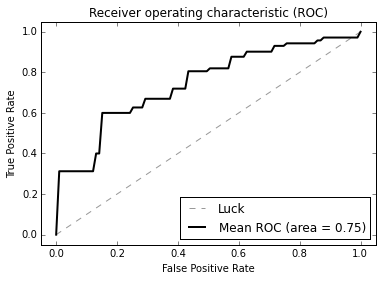
\includegraphics[width=8cm]{svc_linear_cnotopt_normalized_scale64x64.png}
\caption{Receiver operating characteristic (ROC) curve of the average 10-fold cross-validation. The legend show the expected AUC (area under the curve) obtained by luck and the average AUC from the classifier. 67.07\% accuracy of the classifier after normalization and regression of the confounding variables.}
\label{fig_svc_norm_cnotopt}
\end{figure}


If we combine the confound regression with the normalization (unit variance and zero mean for the connectivity of each subject ) and we search for the optimal parameter C for the linear classifier we obtain 69.89\% and an AUC of 0.80 see Figure \ref{fig_svc_norm}.


\begin{figure}[h]
\centering
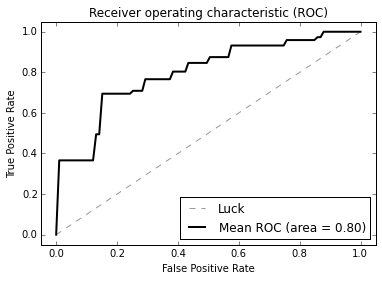
\includegraphics[width=8cm]{svc_linear_normalized_scale64x64.png}
\caption{Receiver operating characteristic (ROC) curve of the average 10-fold cross-validation. The legend show the expected AUC (area under the curve) obtained by luck and the average AUC from the classifier. 69.89\% accuracy of the classifier after normalization and regression of the confounding variables and parameter C optimized.}
\label{fig_svc_norm}
\end{figure}


\subsection{Optimal scale}


\begin{figure}[h]
\centering
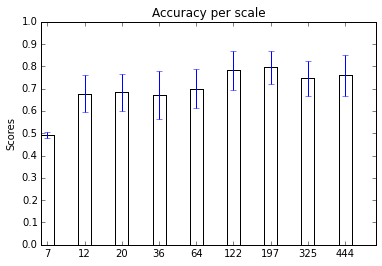
\includegraphics[width=8cm]{acc_scale.png}
\caption{Accuracy scores of the tuned classifier of each functional scale using a 10-fold cross validation.}
\label{fig_scale_svm}
\end{figure}

By selecting the most discriminative scale we where able to achieve a 79.48\% accuracy and a AUC of 0.82 as shown in Figure \ref{fig_svc_norm_optimal_scale}.

\begin{figure}[h]
\centering
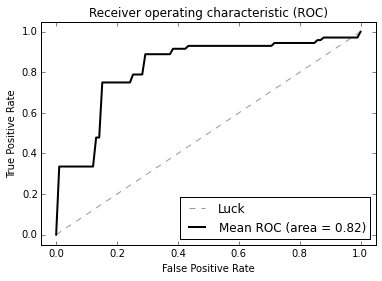
\includegraphics[width=8cm]{svc_linear_normalized_scale197x197.png}
\caption{Receiver operating characteristic (ROC) curve of the average 10-fold cross-validation. The legend show the expected AUC (area under the curve) obtained by luck and the average AUC from the classifier. 79.48\% accuracy of the classifier using features from functional scale 197 after normalization and regression of the confounding variables and parameter C optimized using grid search.}
\label{fig_svc_norm_optimal_scale}
\end{figure}

\subsection{Multiscale}

Using the 3 scales that individually performed the best (namely scale 122, 197 and 444) we obtained an accuracy of $80.14\%$ std $\pm8.36\%$ and an AUC of 0.82 see Figure \ref{fig_svc_bagging_multiscale} for the ROC curve.


\begin{figure}[h]
\centering
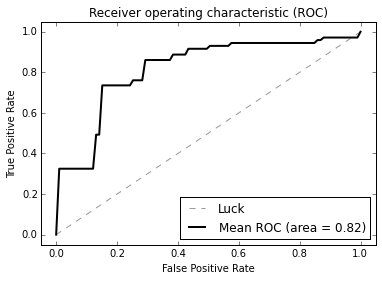
\includegraphics[width=8cm]{svc_linear_multiscale_bagging.png}
\caption{Receiver operating characteristic (ROC) curve of the average 10-fold cross-validation. The legend show the expected AUC (area under the curve) obtained by luck and the average AUC from the classifier. 80.14\% accuracy of the classifier using multiscale bagging from scale 122, 197, 444; after normalization and regression of the confounding variables and parameter C optimized using grid search.}
\label{fig_svc_bagging_multiscale}
\end{figure}

\subsection{I-Relief}

We obtained an accuracy of 73.94\% std $\pm7.41\%$ with an AUC of 0.82 for the optimized pipeline with feature selection based on I-Relief with optimal threshold.

\subsection{Summary}
Table \ref{tab_results} show the results of the experiment described above.


\begin{table}[h]
\begin{tabular}{llll}
\hline
                                   & Accuracy (\%)  & Std (\%)      & AUC           \\ \hline
SVC linear calib 64x64             & 64.53          & 6.86          & 0.70          \\
NC SVC linear 64x64                & 67.07          & 11.08         & 0.75          \\
Opt NC SVC linear 64x64            & 69.89          & 8.69          & 0.80          \\
\textbf{Opt NC SVC linear 197x197} & \textbf{79.48} & \textbf{7.50} & \textbf{0.82} \\
Opt NC SVC rbf 197x197             & 74.61          & 8.75          & 0.80          \\
\textbf{Opt NC Multiscale bagging} & \textbf{80.14} & \textbf{8.36} & \textbf{0.82} \\
Opt NC I-Relief 197x197            & 73.94          & 7.41          & 0.82          \\ \hline
\end{tabular}
\label{tab_results}
\caption{Summary of the performance of each classification pipeline. Acronyms: calib: calibration, NC: normalized and regression of confounds (age and gender), Opt optimisation of the classification parameter using nested 10-fold cross-validation. The multiscale bagging was performed on 3 scales (122, 197 and 444) and I-Relief was perform on the scale 197x197. }
\end{table}

\section{Discussion and Conclusion}

A common mistake made when trying to tackle this kind of problem is to do the feature selection before cross-validation using the labels this may lead in an overestimate of our accuracy. This finding may give very good result that will not generalize well as an example we have done this by running our model with the feature selection procedure (I-Relief) in and out of the cross-validation procedure resulting in improved performance when selecting the features outside the cross-validation loop.

In this study, although not shown in the results section we have tested many other classifier models (SVM with Gaussian kernel, LDA, adaboost, bagging, trees and random forest) none of which perform close to the linear SVM except maybe SVM with Gaussian kernel who obtain 74.61\% accuracy on the best scale (197) using grid search for the optimal parameters. Our hypotheses for the reason why linear SVM work better than more complex classifier is probably due to the fact that the amount of variability in the data make it difficult for higher order classifier to model.  They are more sensitive to outliers and start to focus on noise components that in turn corrupt the classification procedure.

We were able to achieve a decent performance of 79.48\% accuracy using a simple model at the appropriate scale and obtain a 80.14\% accuracy using the multiscale bagging approach. Unfortunately the I-Relief procedure that we proposed to reduce the feature space did not yield as good results as we were anticipating. It was in fact performing worse then the optimal scale using a linear SVM. For the case of the bagging multiscale it may be good to use this procedure instead of the single scale since it as a very similar accuracy but may be more versatile when presented with a different pathology. A major advantage is the fact that we do not need to choose the best scale and it use the power of ensemble methods for it's prediction and therefore may perform better than the single scale in some cases. Future work need to be conducted to assess the performance and generalization potential of the leading models to other datasets and pathologies.

%This project introduce us to the various problematic that one can face in the context of vision and tracking. We were able to achieve the three requirements of the project namely 1) the identification of mobile object and there features, 2) the classification of the object in a two class problem (pedestrian or car) and finally 3) the tracking of the objects across the scene. We also made our software able to identify a trajectory and be able to resolve interference due to two objects crossing path.
%
%An important note relate to the choice of the features for classification, the images use in this project were taken in winter and are not particularly colourful explaining the performance of the 32x32 gray-scale image as equivalent to the RGB one. Event though this choice is acceptable for this particular dataset it will most likely be more appropriate to use a color version for a classifier that would generalized better in other scenery.




% if have a single appendix:
%\appendix[Proof of the Zonklar Equations]
% or
%\appendix  % for no appendix heading
% do not use \section anymore after \appendix, only \section*
% is possibly needed

% use appendices with more than one appendix
% then use \section to start each appendix
% you must declare a \section before using any
% \subsection or using \label (\appendices by itself
% starts a section numbered zero.)
%
%
%
%\appendices
%\section{Proof of the First Zonklar Equation}
%Appendix one text goes here.
%
%% you can choose not to have a title for an appendix
%% if you want by leaving the argument blank
%\section{}
%Appendix two text goes here.

%
%% use section* for acknowledgement
%\ifCLASSOPTIONcompsoc
%  % The Computer Society usually uses the plural form
%  \section*{Acknowledgments}
%\else
%  % regular IEEE prefers the singular form
%  \section*{Acknowledgment}
%\fi


%The authors would like to thank...


% Can use something like this to put references on a page
% by themselves when using endfloat and the captionsoff option.
\ifCLASSOPTIONcaptionsoff
  \newpage
\fi



% trigger a \newpage just before the given reference
% number - used to balance the columns on the last page
% adjust value as needed - may need to be readjusted if
% the document is modified later
%\IEEEtriggeratref{8}
% The "triggered" command can be changed if desired:
%\IEEEtriggercmd{\enlargethispage{-5in}}

% references section

% can use a bibliography generated by BibTeX as a .bbl file
% BibTeX documentation can be easily obtained at:
% http://www.ctan.org/tex-archive/biblio/bibtex/contrib/doc/
% The IEEEtran BibTeX style support page is at:
% http://www.michaelshell.org/tex/ieeetran/bibtex/
\bibliographystyle{IEEEtran}
%
%% argument is your BibTeX string definitions and bibliography database(s)
\bibliography{IEEEabrv,vision,cdansereau}
%
% <OR> manually copy in the resultant .bbl file
% set second argument of \begin to the number of references
% (used to reserve space for the reference number labels box)

%\begin{thebibliography}{1}
%\bibitem{IEEEhowto:kopka}
%H.~Kopka and P.~W. Daly, \emph{A Guide to \LaTeX}, 3rd~ed.\hskip 1em plus
%  0.5em minus 0.4em\relax Harlow, England: Addison-Wesley, 1999.
%
%\bibitem{numpy}
%H.~Kopka and P.~W. Daly, \emph{A Guide to \LaTeX}, 3rd~ed.\hskip 1em plus
%  0.5em minus 0.4em\relax Harlow, England: Addison-Wesley, 1999.
%
%\bibitem{scikit-learn}
%H.~Kopka and P.~W. Daly, \emph{A Guide to \LaTeX}, 3rd~ed.\hskip 1em plus
%  0.5em minus 0.4em\relax Harlow, England: Addison-Wesley, 1999.
%  
%\bibitem{scikit-image}
%H.~Kopka and P.~W. Daly, \emph{A Guide to \LaTeX}, 3rd~ed.\hskip 1em plus
%  0.5em minus 0.4em\relax Harlow, England: Addison-Wesley, 1999.
%
%\bibitem{matplotlib}
%H.~Kopka and P.~W. Daly, \emph{A Guide to \LaTeX}, 3rd~ed.\hskip 1em plus
%  0.5em minus 0.4em\relax Harlow, England: Addison-Wesley, 1999.
%
%\end{thebibliography}


% biography section
% 
% If you have an EPS/PDF photo (graphicx package needed) extra braces are
% needed around the contents of the optional argument to biography to prevent
% the LaTeX parser from getting confused when it sees the complicated
% \includegraphics command within an optional argument. (You could create
% your own custom macro containing the \includegraphics command to make things
% simpler here.)
%\begin{biography}[{\includegraphics[width=1in,height=1.25in,clip,keepaspectratio]{mshell}}]{Michael Shell}
% or if you just want to reserve a space for a photo:
%
%\begin{IEEEbiography}{Michael Shell}
%Biography text here.
%\end{IEEEbiography}
%
%% if you will not have a photo at all:
%\begin{IEEEbiographynophoto}{John Doe}
%Biography text here.
%\end{IEEEbiographynophoto}
%
%% insert where needed to balance the two columns on the last page with
%% biographies
%%\newpage
%
%\begin{IEEEbiographynophoto}{Jane Doe}
%Biography text here.
%\end{IEEEbiographynophoto}

% You can push biographies down or up by placing
% a \vfill before or after them. The appropriate
% use of \vfill depends on what kind of text is
% on the last page and whether or not the columns
% are being equalized.

%\vfill

% Can be used to pull up biographies so that the bottom of the last one
% is flush with the other column.
%\enlargethispage{-5in}



% that's all folks
\end{document}


